\section{Results}

To demonstrate the utility our VTK enhancements provide scientific
visualization efforts and to test various use cases, we have implemented three kinds of
applications for the \texttt{vtkRenderingExternal} approach as well as
a simple example using \texttt{vtkOpenVR}.
Using the Vrui VR integration library, we created the following applications:
GeometryViewer, VolumeViewer and MooseViewer.
As the names suggest, GeometryViewer enables end users to load geometry files from a file; VolumeViewer renders a structured dataset using the GPU based volume rendering technique in VTK; and MooseViewer renders a multi-block unstructured dataset as a geometry or a volume, depending on the end user's interactive selections.

\subsection{Immersive Environments}

A variety of immersive environment display styles exist, from HMDs, to low-cost IQ-stations~\cite{Sherman:2010}, to four- or six-sided CAVE\texttrademark systems. Immersive applications need to support a large number of immersive environments, as each has its strength and applicability in real-world scenarios. We have tested our work in the following virtual environments: 

\begin{compactitem}
\item a four-sided CAVE\texttrademark;
\item a low cost IQ-station; and 
\item an HTC VIVE HMD.
\end{compactitem}

In the first two cases, the \texttt{vtkRenderingExternal} module was used with the Vrui VR toolkit to provide the configuration necessary to run the application. For HTC VIVE, we leveraged \texttt{vtkOpenVR}. 

\subsection{Vrui Implementation}

The task of a VR toolkit is to shield an application developer from the particular configuration of an immersive environment, such that applications can be developed quickly and in a portable and scalable fashion. There are three important parts of this overarching goal: encapsulation of the display environment, encapsulation of the distribution environment and encapsulation of the input device environment.

The Vrui VR toolkit supports fully scalable and portable applications that run on a range of immersive environments, starting from laptops with touchpads, to desktop environments with special input devices such as space balls, to full-blown immersive VR environments ranging from single-screen workbenches to multi-screen tiled display walls or CAVE\texttrademark systems. Applications using the Vrui VR toolkit are written without a particular input environment in mind, and Vrui enabled immersive environments are configured to map the available displays and input devices to the application, such that they appear to be written natively for the environment. For example, a Vrui application running on the desktop should be as usable and intuitive as any 3D application written specifically for the desktop.

We developed some example applications that serve as validation of this effort. There is an example within the VTK source tree for the \texttt{vtkRenderingExternal} module that renders a VTK sphere in an OpenGL Utility Toolkit (GLUT) window. We also developed three advanced applications that illustrate VTK rendering within a Vrui created OpenGL context. These applications exhibit varying capabilities of the VTK infrastructure leveraged by the \texttt{vtkRenderingExternal} module. 

\subsubsection{GeometryViewer}

\begin{figure}[h!]
 \centering
 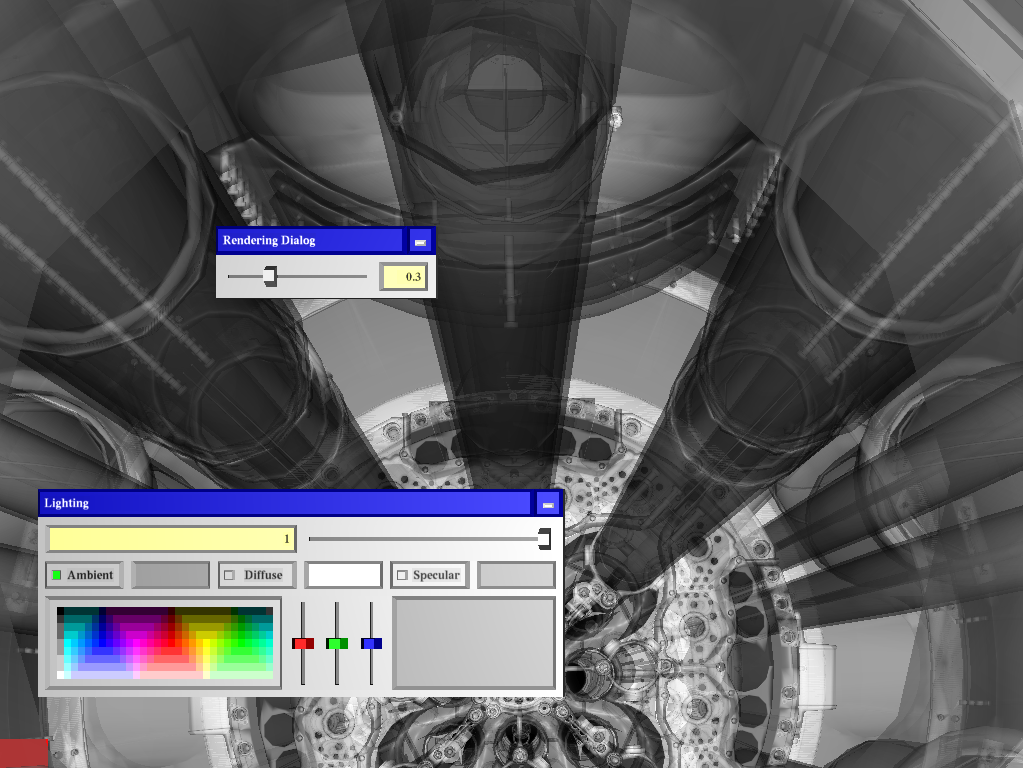
\includegraphics[width=3.5in]{images/vessel.png}
 \caption{Geometry representing Idaho National Laboratory's Advanced Test Reactor (ATR) core. The geometry is used to virtually understand maintenance processes in this extreme environment.}
 \label{fig:vessel}
\end{figure}

GeometryViewer~\cite{GeometryViewer} reads and renders a Wavefront (.obj) file that defines a geometry.
It reads the file using the standard \texttt{vtkOBJFileReader} that creates \texttt{vtkPolyData} from the geometry.
The \texttt{vtkPolyData} is then mapped, using the polydata rendering pipeline in VTK, as a \texttt{vtkActor} object.
The main menu of the application allows the user to center the geometry to the screen as well as to change its representation.
The \textit{Center Display} button calculates the transformation from the current camera position and direction to the center position.
The \textit{Rendering Options} sub-menu allows the end user to change the opacity of the \textit{vtkActor} object, leveraging our work on dual depth peeling, as well as its representation to either the points, the wireframe or the surface.
In addition to VTK level modifications, the application has support for OpenGL level widgets (e.g., \texttt{glClipPlane}).
This shows that native OpenGL operations can also be interactively performed when using the VTK rendering pipeline.

In Figure~\ref{fig:vessel}, we show the Vrui user interface (UI) with the ``\textit{Rendering Options}" dialog that allowed us to adjust the transparency of the Advanced Test Reactor (ATR) core. In addition, we used the Vrui UI to build an interface for the lighting color that seamlessly maps between Vrui and VTK.

This example has the functionality contained in the integration between Vrui and Delta3D presented in Sherman et al.~\cite{Sherman:2010}. Both applications were simple to develop, but the performance of GeometryViewer is faster, especially when rendering transparent geometry. In addition, GeometryViewer integrates the lighting between the VR toolkit and VTK, in contrast to the Vrui/Delta3D integration, which requires modification to the material textures to provide false lighting.

\subsubsection{VolumeViewer}

\begin{figure}[h!]
 \centering
 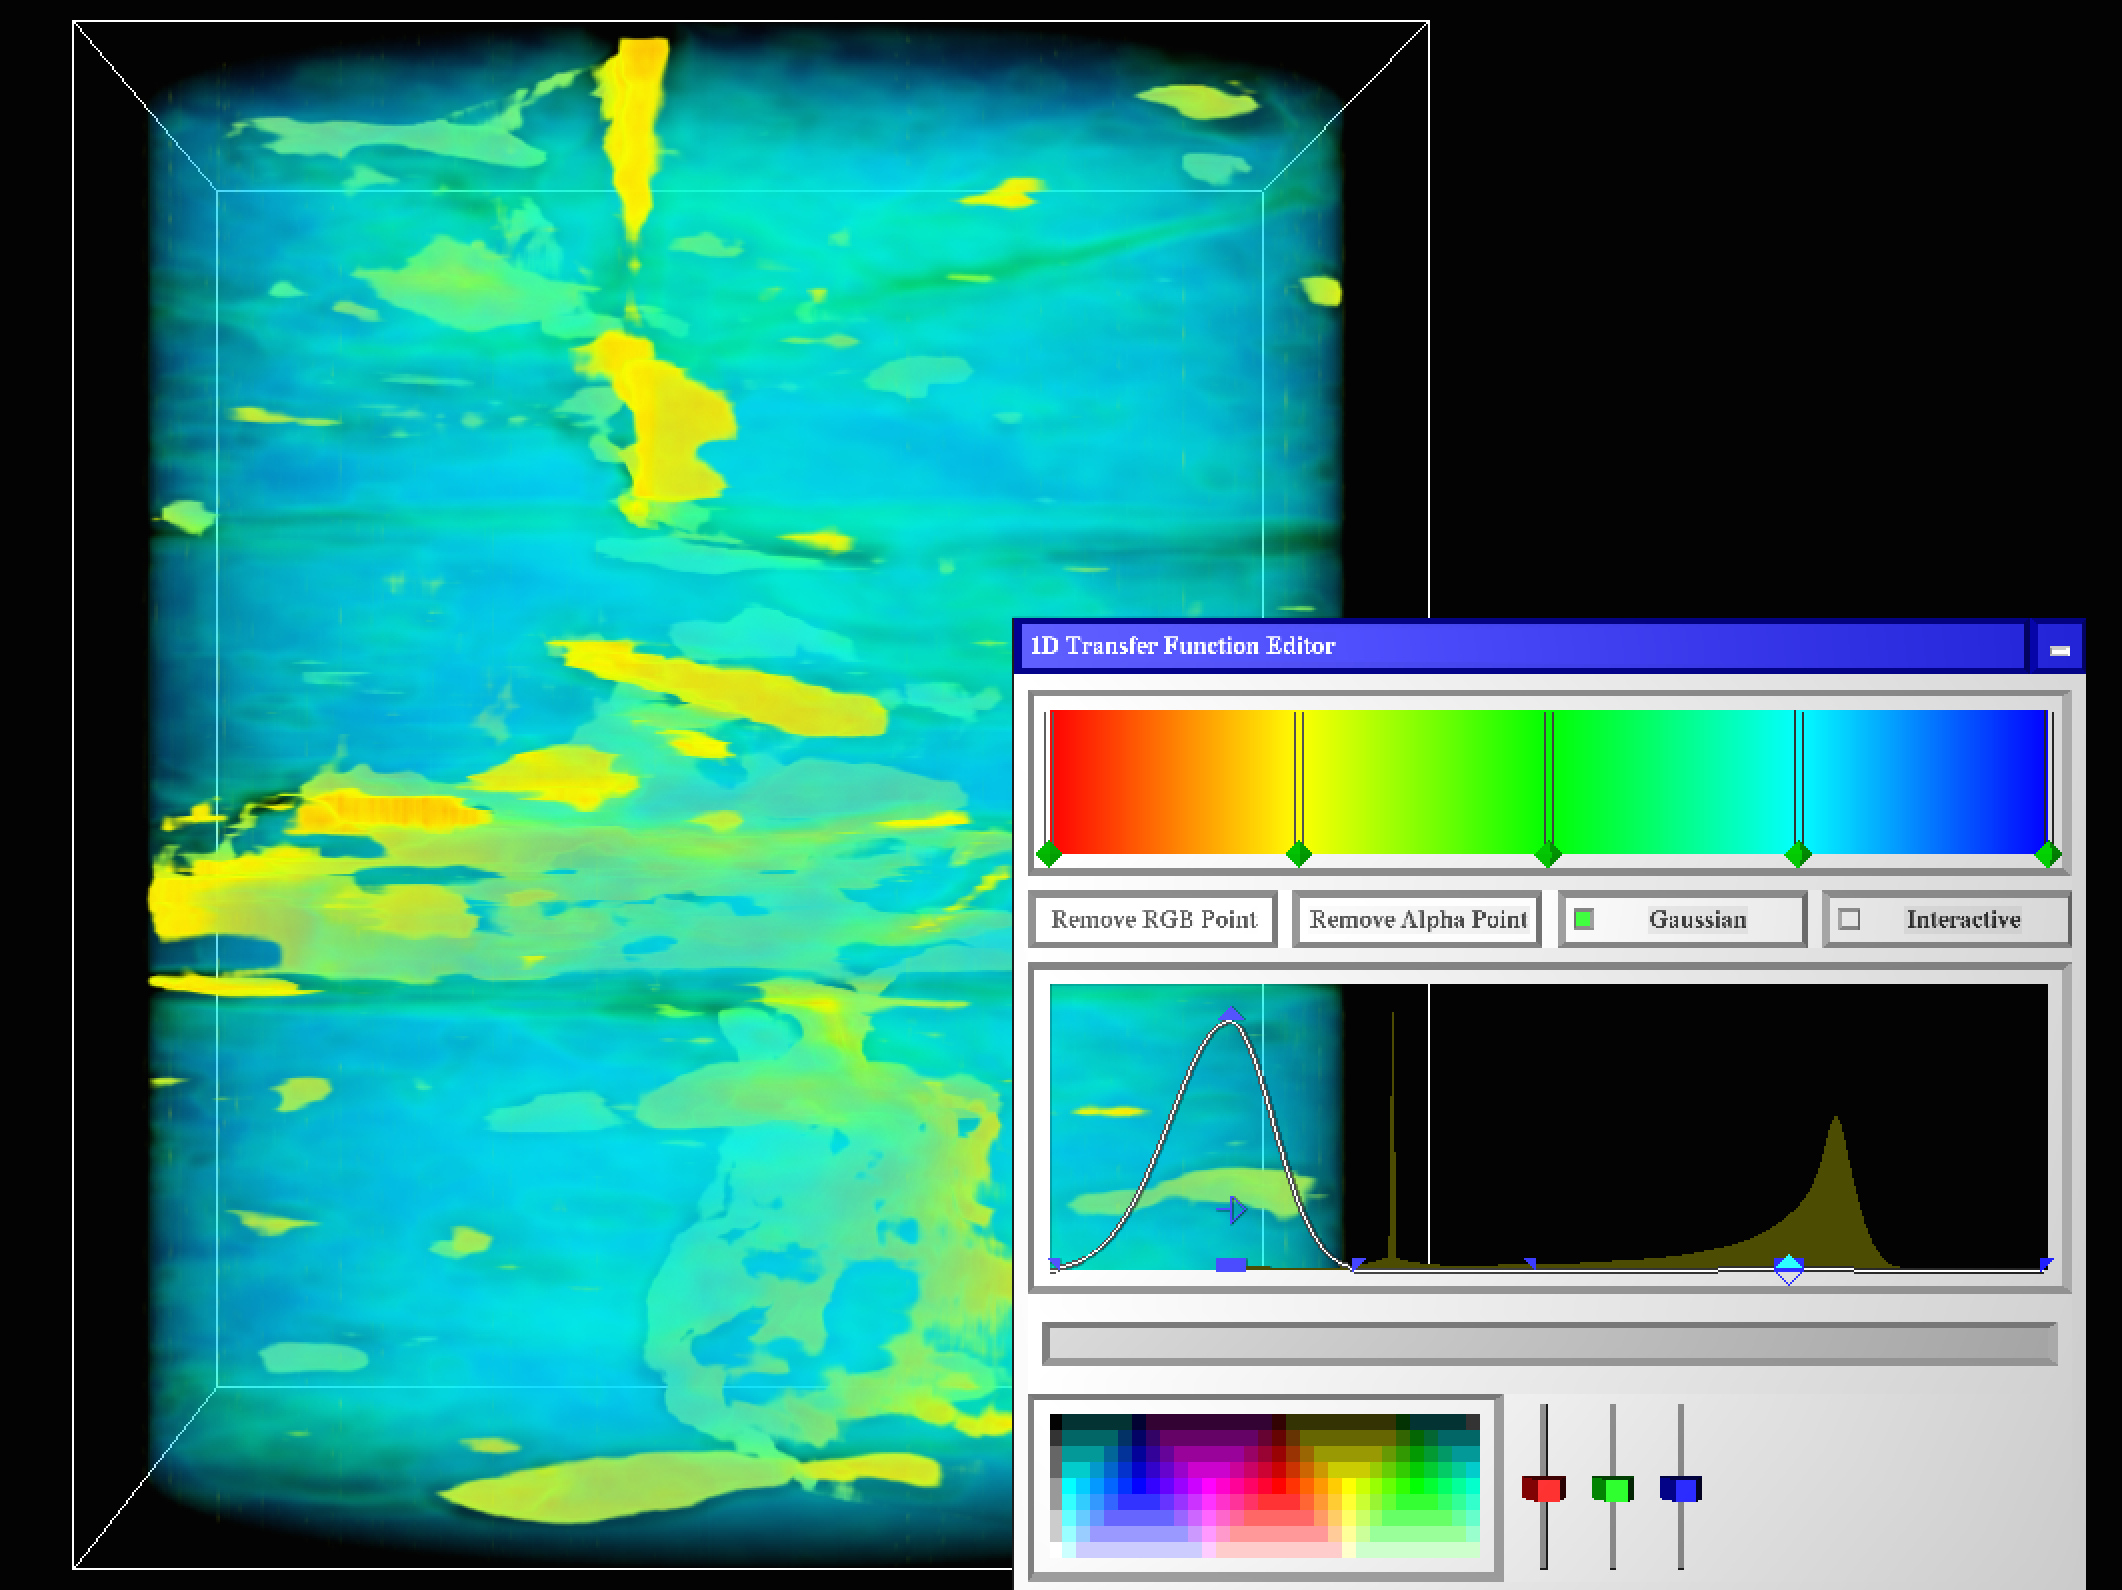
\includegraphics[width=3.5in]{images/rock-transferfunction.png}
 \caption{A digitized well ``rock" core. The yellow isosurfaces isolate the oil trapped within the shale rock.}
 \label{fig:volume}
\end{figure}

VolumeViewer~\cite{VolumeViewer} reads and renders VTK ImageData (.vti) files that define structured points datasets.  The application instantiates a pipeline that allows volume rendering of the dataset. Several pre-defined color maps help to change the mapping of scalar values to colors. A \textit{Transfer Function} editor allows changes to be made to the color and opacity of the rendered volume.

Figure~\ref{fig:volume} depicts our implementation of a ``\textt{Transfer Function} editor using the Vrui UI. In addition, we leveraged \texttt{vtkFlyingEdges3D} to display the oil isosurfaces in yellow and blend the results in the volume.

Widgets such as \texttt{Isosurfaces}, \texttt{Contours} and \texttt{Slice} provide VTK level operations that can be carried out on the dataset. To circumvent possible interaction problems when dealing with large datasets, a low-resolution mode is provided that downsamples the dataset. This lets the end user fulfill actions quickly and then revert back to the full size, when they are ready to visualize the complete dataset.

Immersive volume visualization applications are fundamental for a number of scientific research domains, and it is not surprising that there exists a number of partial solutions in the public domain. VolumeViewer has similar features contained in both Visualizer~\cite{Billen:2008} and Toirt Samhlaigh~\cite{O'Leary:2008}. Both applications use complex, from scratch, OpenGL algorithms that were time-consuming to develop. Visualizer uses a standard GPU OpenGL Shading Language (GLSL) shader-based ray-casting algorithm. Toirt uses an octree-based space-skipping GPU GLSL shader-based view-aligned algorithm to provide higher performance on larger volumes. In contrast, VolumeViewer requires less than a hundred lines of VTK API to implement roughly the same GPU GLSL shader-based ray casting used in Visualizer. The performance of VolumeViewer is equal to or exceeds that of the other tools. In addition, by modifying a line or two of VolumeViewer code, the application can accept data from any of the hundred-plus supported scientific data formats|a feat that would require the implementation of readers, data structures and algorithms in either of the other two applications.

\subsubsection{MooseViewer}

\begin{figure}[h!]
 \centering
 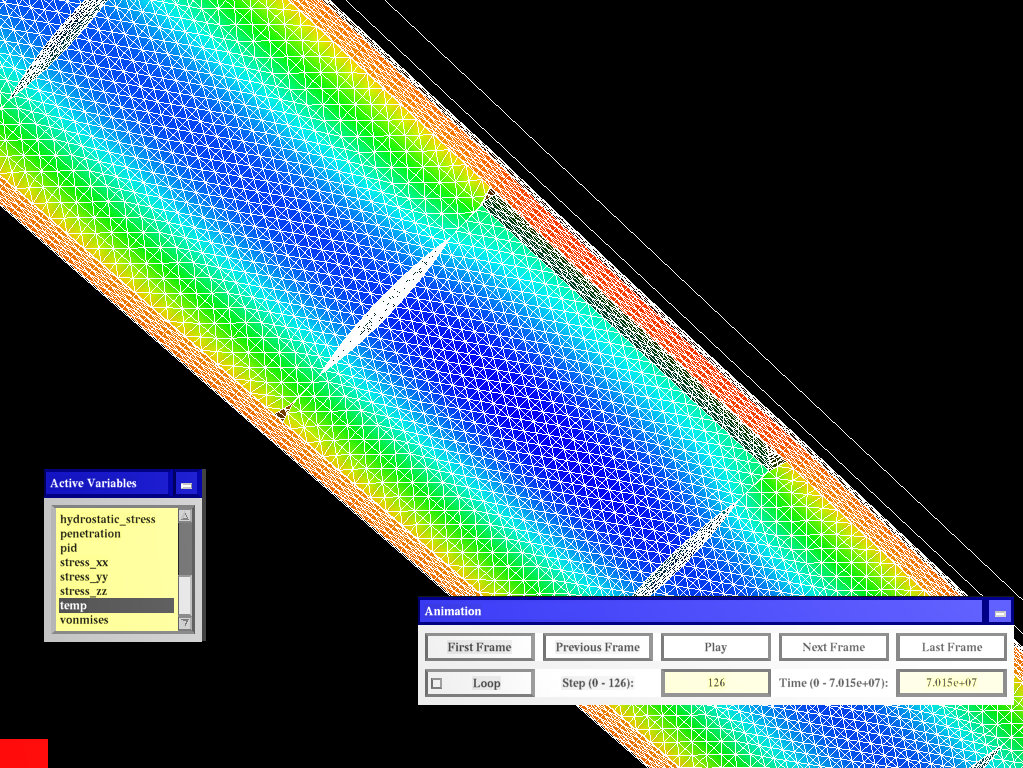
\includegraphics[width=3.5in]{images/fuelpin.png}
 \caption{A MOOSE Framework application, BISON, simulates a nuclear pin with missing cladding on one of the fuel pellets.}
 \label{fig:fuelpin}
\end{figure}

MooseViewer~\cite{MooseViewer} reads and displays Moose framework~\cite{Gaston:2015, MooseFramework} ExodusII (.ex2, .e) files in immersive environments. The application uses \texttt{vtkExodusIIReader} to read geometry defined in ExodusII files as well as associated attributes (e.g., temperature, burnup, etc.). The application permits only user-selected variables to be loaded as data arrays, thus reducing memory overhead. A ``\textit{Color By}" sub-menu is dynamically populated with user-selected variables. The sub-menu maps the chosen variable scalars to colors using the selected color map.
An interesting capability of the application is animation of the dataset over time.
The ``\textit{Animation}" dialog helps play through the time steps with controls for looping and stepping through the time steps.

In Figure~\ref{fig:fuelpin}, we see surface geometry colored by the selected temperature attribute animated using the ``\textit{Animation}" dialog.

\begin{figure}[h!]
  \centering
  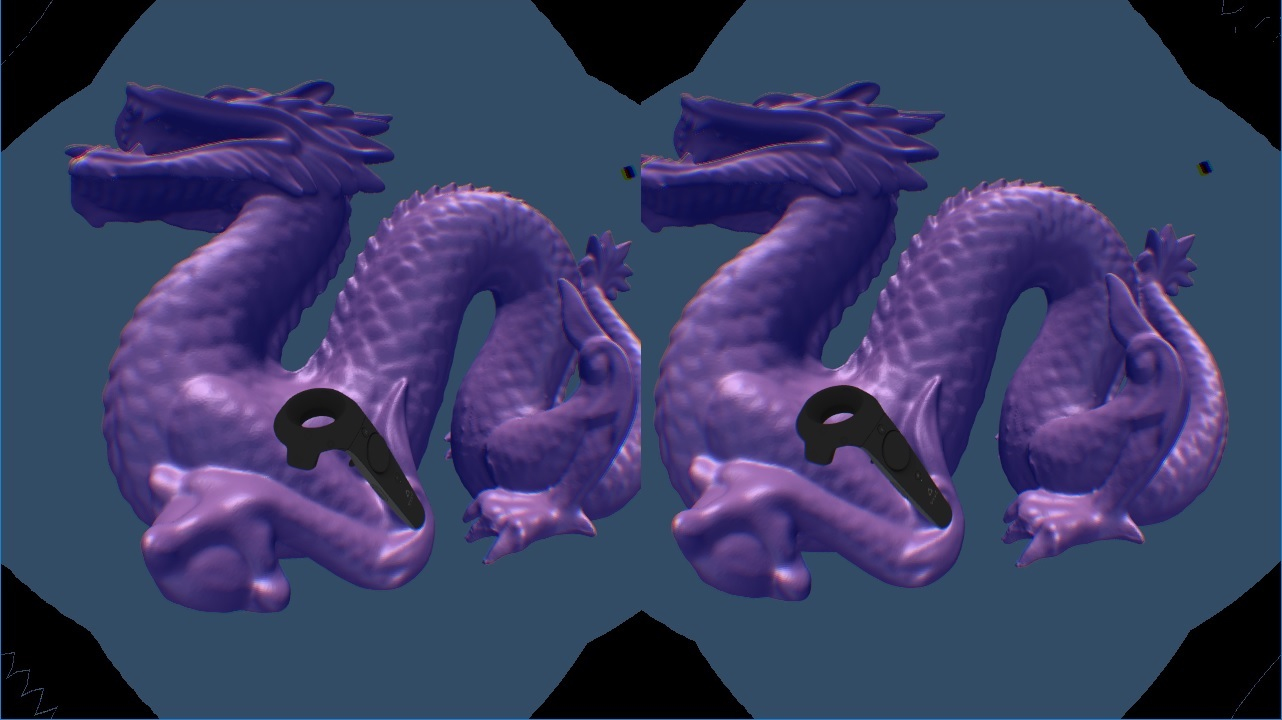
\includegraphics[width=3.5in]{images/Dragon.jpg}
  \caption{A polygonal rendering of a sample dataset by VTK for OpenVR on HTC Vive.}
  \label{fig:openvrdragon}
\end{figure}

Like Visualizer~\cite{Billen:2008}, MooseViewer provides a number of scientific visualization techniques for simulation data, but MooseViewer was created in weeks. Enhancements are added by simply plugging in alternative VTK algorithms to increase/scale performance.  Although it is focused on the ExodusII file format, MooseViewer makes accepting data from other scientific data formats a simple task. MooseViewer outperforms Visualizer using the VTK OpenGL 3.2+ rendering pipeline, but pure rendering performance fails to highlight the unique immersive-specific level-of-detail algorithms in Visualizer. Visualizer is a fantastic immersive application. If an end user has data in one of its accepted formats, we encourage that person to leverage some of the unique Visualizer features.

%\begin{figure}[h!]
%  \centering
%  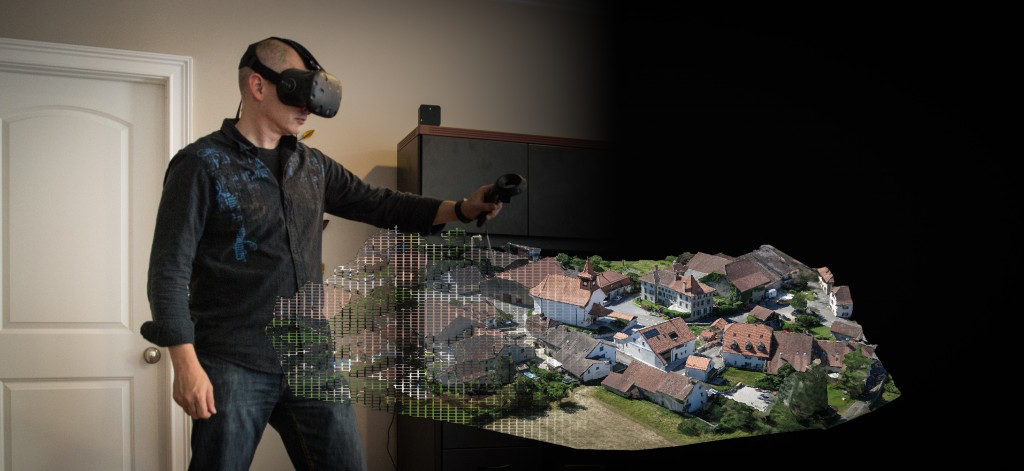
\includegraphics[width=3.5in]{images/ViveTownData.png}
%  \caption{HTC Vive Town using VTK with OpenVR.}
%  \label{fig:ViveTown}
%\end{figure}

\subsection{OpenVR Implementation}

This example creates a trivial VTK pipeline that reads a polygonal geometry file
using the \texttt{vtkPLYReader} and maps it to the scene using the above described \texttt{vtkOpenVR}
classes. As seen in Figure \ref{fig:openvrdragon}, the rendering
classes created a stereo pair from the view and warped it to the HTC Vive camera model. 
The example is available as a test case under the
\texttt{vtkOpenVR} module in the VTK source.

The modest amount of code needed to put VTK generated polygons into the
Vive HMD attests to the modularity and complete integration of the
existing VR framework|in this case, \texttt{vtkOpenVR}.
